\documentclass{standalone} 
\usepackage{amsmath,amssymb,amsthm}
\usepackage[usenames,dvipsnames,table]{xcolor}
\usepackage{tikz} \usetikzlibrary{calc,arrows.meta,intersections,patterns}

%% !TEX root = ThesisManuscript_SJ.tex
%%
%%
%%	MY COLORS
%%_______________________________________________
\definecolor{MyBlue}{RGB}{0,120,155}
\definecolor{MyDarkBlue}{rgb}{0, 0.25, 0.45}
\definecolor{MyBrown}{rgb}{0.28, 0.20, 0.20}
\definecolor{MyOrange}{RGB}{255,80,30}
\definecolor{MyOldOrange}{rgb}{0.75, 0.25, 0.0}
\definecolor{MyRed}{RGB}{200,0,0}
\definecolor{MyGray}{RGB}{200,200,200}
\definecolor{MyGreen}{rgb}{0.33, 0.5, 0.18}
\definecolor{MyDarkGreen}{rgb}{0.15, 0.25, 0.18}
\definecolor{MyTurquoise}{rgb}{0, 0.4, 0.4}
\definecolor{MyViolet}{rgb}{0.44, 0.16, 0.39}
\definecolor{MyYellow}{rgb}{1, 0.65, 0}

\tikzstyle{dark_top} 	= [rectangle, draw = none, text = white, fill=MyOldOrange]
\tikzstyle{dark_bottom} = [rectangle, draw=none, text width=4.5cm, text = white, fill=MyDarkBlue]
\tikzstyle{light_bottom} = [rectangle, draw=none, text width=4.5cm, text = black, fill=MyDarkBlue!20]
\tikzstyle{dark_right}	= [rectangle, draw=none, text = white, fill=MyTurquoise]
\tikzstyle{light_right} 	= [rectangle, draw=none, text = MyTurquoise, fill=MyTurquoise!20]
\tikzstyle{dark_left} 	= [rectangle, draw=none, text = white, fill=MyGreen]
\tikzstyle{light_left} 	= [rectangle, draw=none, text = MyGreen!95!black, fill=MyGreen!20]
\tikzstyle{smalltext} = [rectangle, draw=none,minimum height=1cm, yshift=-0.5cm]
		
\begin{document}
\begin{tikzpicture} [node distance=1cm, rounded corners=2pt, text width=3.2cm, minimum height=1.1cm, align=center, outer sep=4pt, line width=1.5pt]
	% TOP
	\node (risk)  [dark_top] 										{Perceived \\ \smallskip 
															{risk of infection}};
	% BOTTOM
	\node (cov) [below of=risk,yshift=-1.5cm,dark_bottom, text width=2.5cm] 	{Prevention \\ \smallskip 
															coverage};
	% LEFT
	\node (Ind_Def)  [below of=risk, xshift=-4.5cm,yshift=-1.5cm,dark_left] 		{ Individual's decision};
	\node (Ind_Graph) [below of=Ind_Def,yshift=-1.5cm]  				{
\includegraphics[width=\linewidth]{Fig_Dilemma.png}};
	\node (Ind_mod_by)  [below of=Ind_Graph,yshift=-1cm] 				{\small modeled by a};
	\node (Ind_Mod)  [below of=Ind_mod_by,yshift=0.3cm,light_left] 		{Game-theoretic \\ model};
	% RIGHT	
	\node (Pop_Def) [below of=risk, xshift=4.5cm,yshift=-1.5cm,dark_right] 	{Epidemic dynamics};
	\node (Pop_Graph) [below of=Pop_Def,yshift=-1.5cm]  				{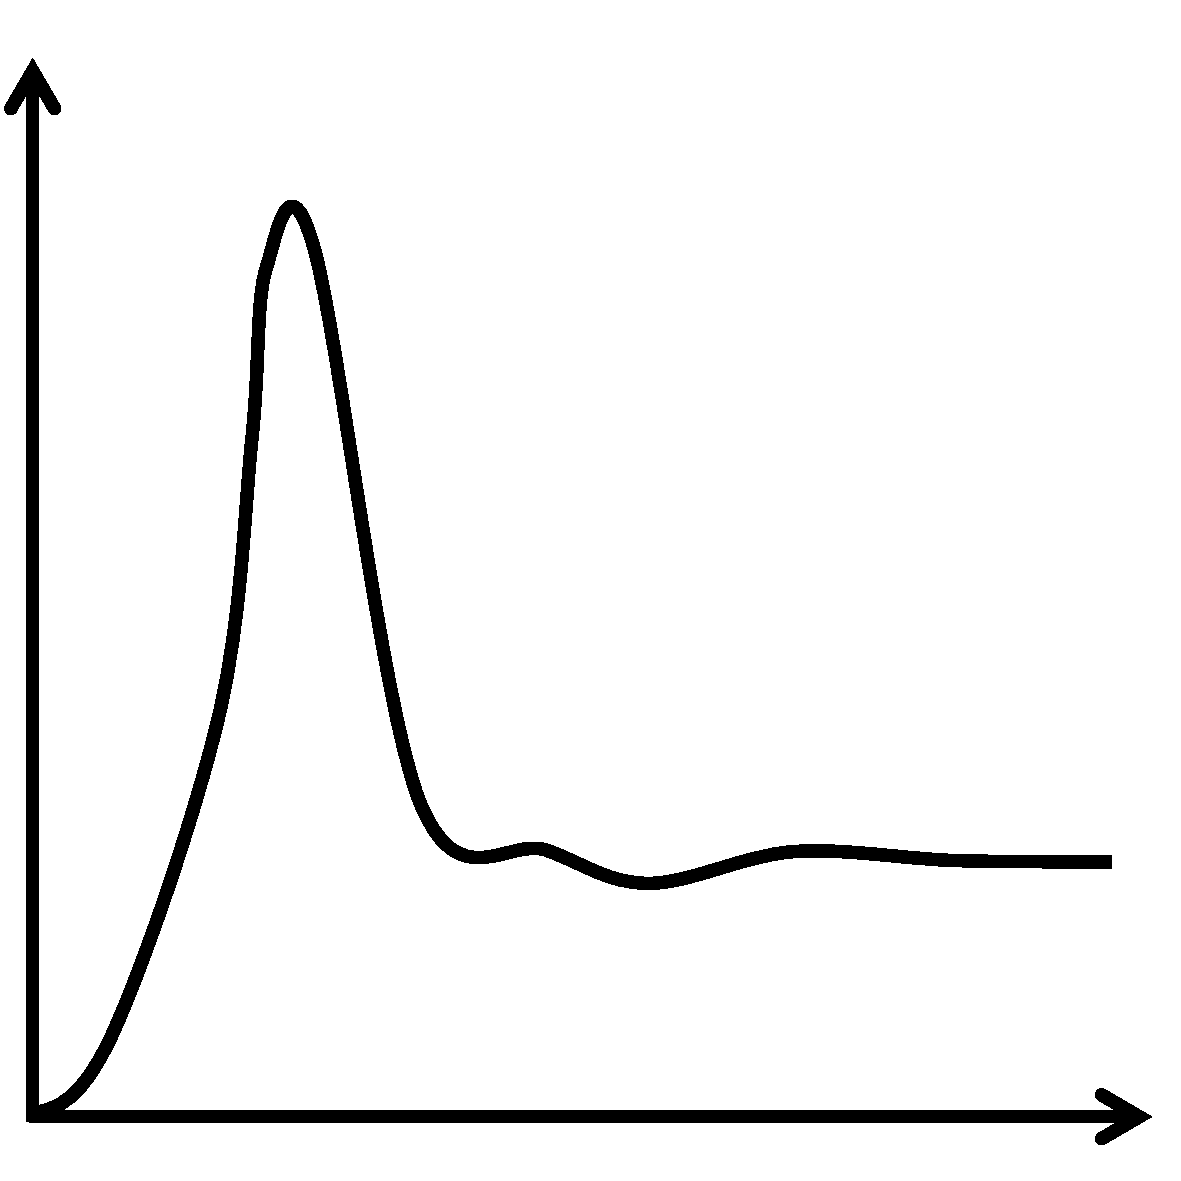
\includegraphics[width=\linewidth]{Epidemic.pdf}};
	\node (Pop_mod_by)  [below of=Pop_Graph,yshift=-1cm, text = MyBrown] {\small modeled by a};
	\node (Pop_Mod) [below of=Pop_mod_by,yshift=0.3cm,light_right] 		{Compartmental model};

	% ARROWS
	\draw[bend right,->] (risk.west) to (Ind_Def);
	\draw[bend left,<-] (risk.east) to (Pop_Def);
%	\draw[bend right,->, color=MyBrown](risk.west) to node [text width=2cm,anchor=east,pos=0.5,xshift=-1cm] {\Large influences} (Ind_Def);
%	\draw[bend left,<-,color=MyBrown]  	(risk.east) to node [text width=2cm,anchor=west,pos=0.5,xshift=0.5cm]  {\Large defines} (Pop_Def);
	
	\draw [->] (Ind_Def)  --  (cov);
	\draw [->] (cov) --  (Pop_Def);		
%	\draw [->] (cov) -- node [text width=3cm,anchor=south,yshift=-0.4cm,pos=0.5] {\small \& other \\ factors} (Pop_Def);		
 \end{tikzpicture}
\end{document}

